%%
% Please see https://bitbucket.org/rivanvx/beamer/wiki/Home for obtaining beamer.
%%
%\documentclass[11pt,aspectratio=169]{beamer}
%\documentclass[11pt,aspectratio=169,xcolor={dvipsnames}]{beamer}

\documentclass[11pt,aspectratio=169,xcolor={dvipsnames},hyperref={pdftex,pdfpagemode=UseNone,hidelinks,pdfdisplaydoctitle=true},usepdftitle=false]{beamer}
\usepackage{presentation}


\title{Lecture 15: Empirical Credit Supply}
\author{Juan Herre\~{n}o\\UCSD}
\date{2026}

% Enter presentation title to populate PDF metadata:
\newcommand{\Cov}{\text{Cov}_\lambda}
\newcommand{\El}{\mathbb{E}_\lambda}
\newcommand{\mm}{\text{{\fontfamily{qzc}\selectfont m}}}
\usepackage{cancel}
\usepackage{booktabs}
\begin{document}

\maketitle


\begin{frame}{Motivating Facts}
\begin{itemize}
\item Take the Great Depression
\begin{itemize}
\item On one side, waves of bank failures, culminating with the shutdown of the banking system in March 1933.
\item On the other side, high rates of layoffs and bankruptcy in the real sector
\end{itemize}
\item Coincidence in timing
\begin{itemize}
\item The first banking crisis 1930 stalled the initial recovery
\item New slump after a bank panic in 1931
\item The economy and the banking sector reached lows in 1933.
\end{itemize}
\end{itemize}
Was this an unlucky coincidence, or did cuts in lending supply damage the economy?
\end{frame}

\begin{frame}{Motivation}
\begin{itemize}
\item Causal effects of shocks to the banking sector on firms
\item You can think of it as a joint hypothesis
\begin{itemize}
\item Banks pass-through their shocks to their lenders (bank-lending channel)
\item Firms cannot find alternatives to bank lending (firm-borrowing channel)
\end{itemize}
\end{itemize}
\end{frame}


\begin{frame}{Simplest Regression}
\begin{itemize}
\item Think of a panel of firms producing $Y_i$ and borrowing $Q_i$
\item $\Delta$ computes the difference between a pre-recession to recession period
\[\Delta \log Y_i = \beta_0 + \beta_1 \Delta \log Q_i + \epsilon_i\]
\item What is $\hat{\beta_1}$ measuring?
\end{itemize}
\end{frame}

\begin{frame}{Intuitive identification challenge}
\[\Delta \log Y_i = \beta_0 + \beta_1 \Delta \log Q_i + \epsilon_i\]
\begin{itemize}
\item Reverse causality: Not only shifts to credit supply in the data, but also to credit demand
\begin{itemize}
\item Firms that produce more, may need to raise additional credit
\end{itemize}
\item Omitted Variables bias: Future investment opportunities may drive both $\mathbb{E}(\epsilon_i \Delta \log Q_i) \neq 0$
\end{itemize}
Theoretical basis for $\beta_1 > 0$: Bernanke Gertler (1989), among others: Shifts in financial variables impair non-financial production
\end{frame}

\section{Khwaja and Mian 2008}
\begin{frame}{Khwaja and Mian 2008}
\begin{itemize}
\item Context: Nuclear tests in Pakistan in 1998 triggered sanctions
\item Government stopped USD deposit convertibility
\begin{itemize}
\item Convertibility: Convert one asset (deposits) into another (cash)
\end{itemize}
\item Not unusual. The American banking system suspended convertibility several times in the XIX and early XX century
\item The key references on bank runs and suspension of convertibility are
\begin{itemize}
\item Bryant 1980
\item Diamond Dybvig 1983
\item Gorton 1985
\end{itemize}
\end{itemize}
\end{frame}


\begin{frame}{Khwaja and Mian 2008}
\begin{itemize}
\item USD deposits widely popular
\item But heterogeneous across banks. Not obviously random.
\item Savers deposited USD in commercial banks. Commercial banks sent USD to the CB in exchange for rupees. When a depositor demanded their deposits back, the CB handed the dollars to the commercial bank at the \textit{time of deposit} exchange rate in exchange for rupees.
\item Reform after massive depreciation
\begin{itemize}
\item Government allowed demand deposits back at the current (worse) exchange rate
\item Partial default on dollar deposits
\item Savers lost confidence and demanded their deposits back. Differential liquidity shock to banks who received USD deposits
\end{itemize}
\end{itemize}
\end{frame}

\begin{frame}{Khwaja and Mian 2008}
\begin{figure}
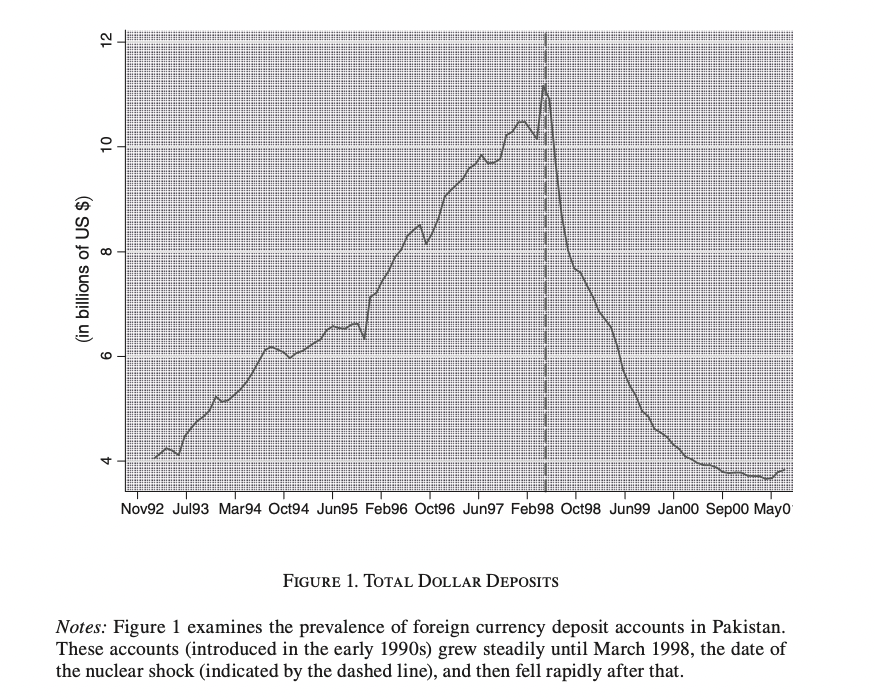
\includegraphics[scale=0.25]{figures/km_1}
\end{figure}
\end{frame}


\begin{frame}{Khwaja and Mian 2008}
\begin{figure}
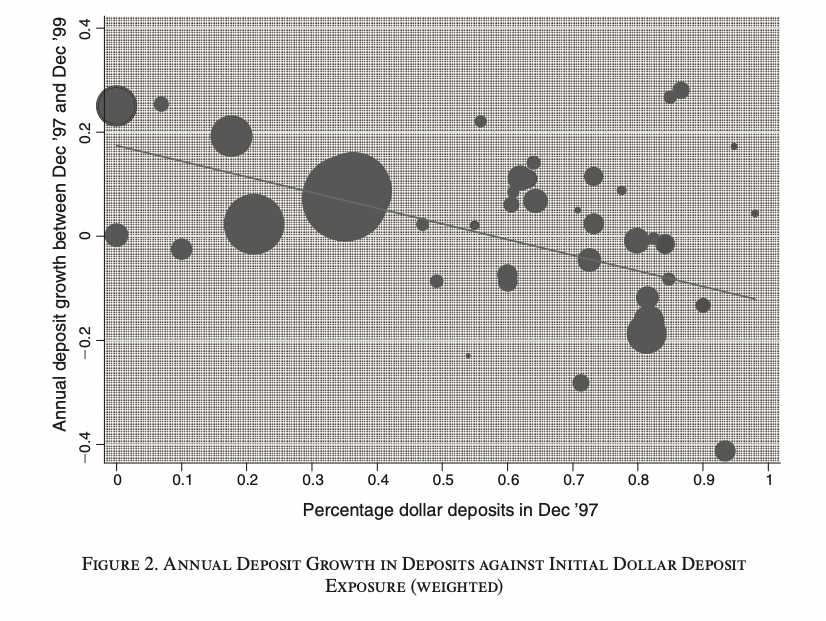
\includegraphics[scale=0.25]{figures/km_2}
\end{figure}
\end{frame}


\begin{frame}{Empirical Specification}
Do balance sheet shocks to banks pass-through to firm borrowing?
$$\Delta Q_{ij} = \beta_j + \beta_1 \Delta D_i + \epsilon_{ij}$$
\begin{itemize}
\item $Q_{ij}$ loan size of a firm-bank pair
\item $\beta_j$ firm fixed effect
\item $\Delta D_i$ change in bank-level dollar-denominated deposits
\item This firm-fixed effect approach became the standard in the literature
\end{itemize}
\end{frame}

\begin{frame}{Empirical Specification}
\begin{itemize}
\item Effectively uses only multi-bank firms
\item The firm fixed effect soaks any shock that causes changes in overall firm credit
\item How much firms increase their borrowing from one bank relative to another bank
\item What could go wrong?
\end{itemize}
\end{frame}

\begin{frame}{The null hypothesis}
$$\Delta Q_{ij} = \beta_j + \beta_1 \Delta D_i + \epsilon_{ij}$$
\begin{itemize}
\item What is the economic meaning of the null hypothesis $H_0 : \beta_1 = 0$?
\item Think of two worlds in which $\beta_1 = 0$. Thoughts?
\end{itemize}
\end{frame}

\begin{frame}{Identifying assumption}
\begin{itemize}
\item Recall
$$\Delta L_{ij} = \beta_j + \beta_1 \Delta D_i + \epsilon_{ij}$$
\item What we need to assume
$$\mathbb{E}(\Delta D_i  \epsilon_{ij}) = 0$$
\item What does it mean?
\item Construct a scenario that breaks the assumption
\end{itemize}
\end{frame}

\begin{frame}{Results}
\begin{figure}
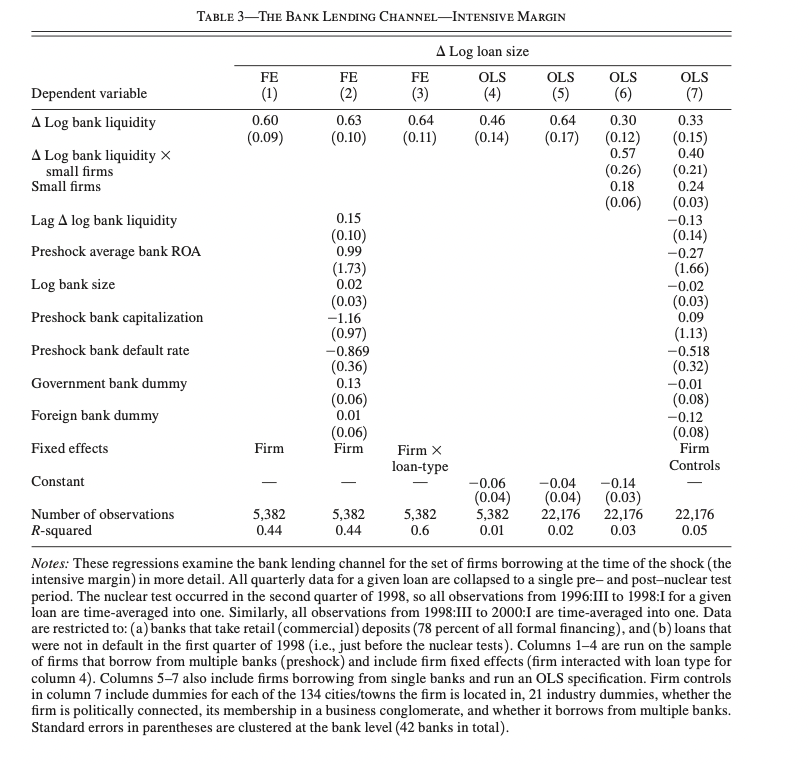
\includegraphics[scale=0.3]{figures/km_3}
\end{figure}\end{frame}


\begin{frame}{Results}
\begin{figure}
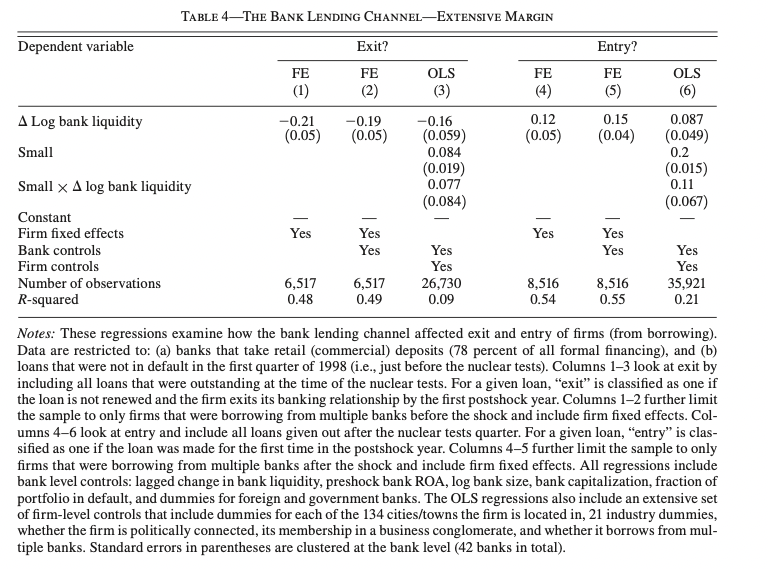
\includegraphics[scale=0.35]{figures/km_4}
\end{figure}
\end{frame}



\begin{frame}{Relation to Chodorow-Reich 2014}
\begin{itemize}
\item Khwaja-Mian (2008) mostly about financial variables
\item In particular credit demand
\item Need variation within the firm
\item But are credit effects relevant at the firm level?
\item Aggregate bank-firm results at the firm level
\end{itemize}
\end{frame}


\begin{frame}{Chodorow-Reich 2014}
\begin{itemize}
\item Casual observation suggests the Lehman bankruptcy changed the scope of the Great Recession (Blinder 2013)
\item Corporate paper markets, interbank lending, lending supply froze
\item Many of these effects were national (even global) driven by panic/pessimism/...
\item The recession turned from a Wall Street problem into a Main Street problem after September 15th, 2008
\item But is there a causal link from drops in lending to drops in employment?
\item Idea: look at firms with differential exposure to Lehman
\end{itemize}
\end{frame}


\begin{frame}{Variation across firms}
\begin{itemize}
\item Start by measuring the cut in lending by bank $b$
\item $L_{b,j,t}$ The loans given by bank $b$ to firm $j$ in period $t$
\item Leave-one-out growth in bank credit
$$\Delta L_{-i,b} = \frac{\sum_{i \neq j} \alpha_{b,j,crisis} L_{b,j,crisis}}{\sum_{i \neq j} \alpha_{b,j,normal} L_{b,j,normal}}$$
\item Aggregate for firm $i$ across banks $b$
$$\Delta \tilde{L}_{i,s} = \sum_{b \in s} \alpha_{b,i,last} \Delta L_{-i,b}$$
\item Shift-share design. Bank-level shocks, firm-level exposure
\end{itemize}
\end{frame}


\begin{frame}{Firm-bank relationships are sticky - Suggests room for a strong first stage}
\begin{figure}
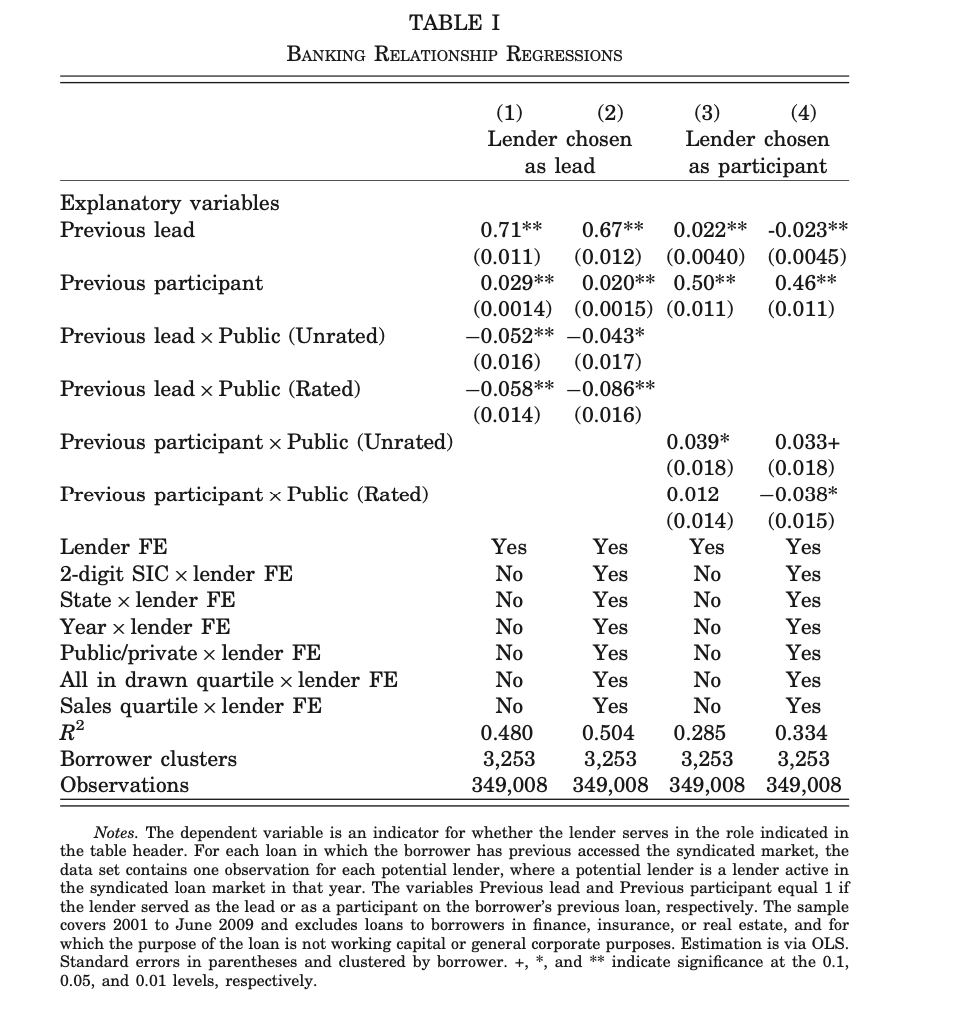
\includegraphics[scale=0.45]{figures/cr_1}
\end{figure}
\end{frame}

\begin{frame}{IV First Stage}
\begin{figure}
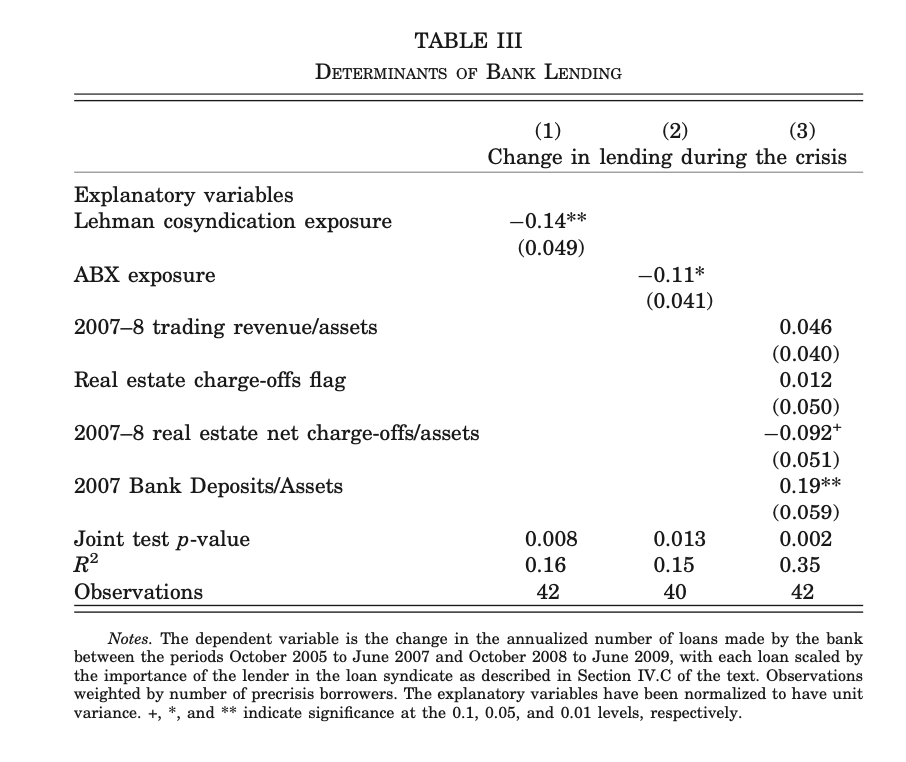
\includegraphics[scale=0.45]{figures/cr_2}
\end{figure}
\end{frame}


\begin{frame}{Results on Rates - Suggests credit supply disruptions}
\begin{figure}
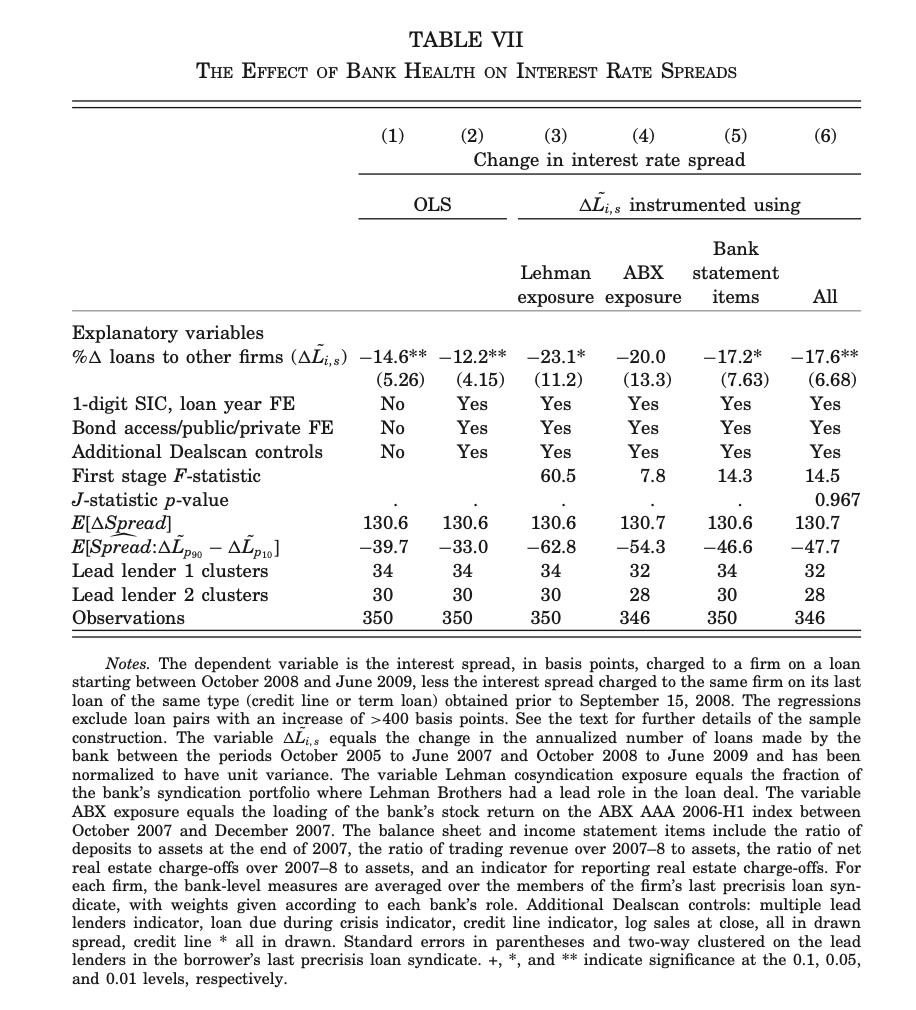
\includegraphics[scale=0.45]{figures/cr_3}
\end{figure}
\end{frame}


\begin{frame}{Results on Employment}
\begin{figure}
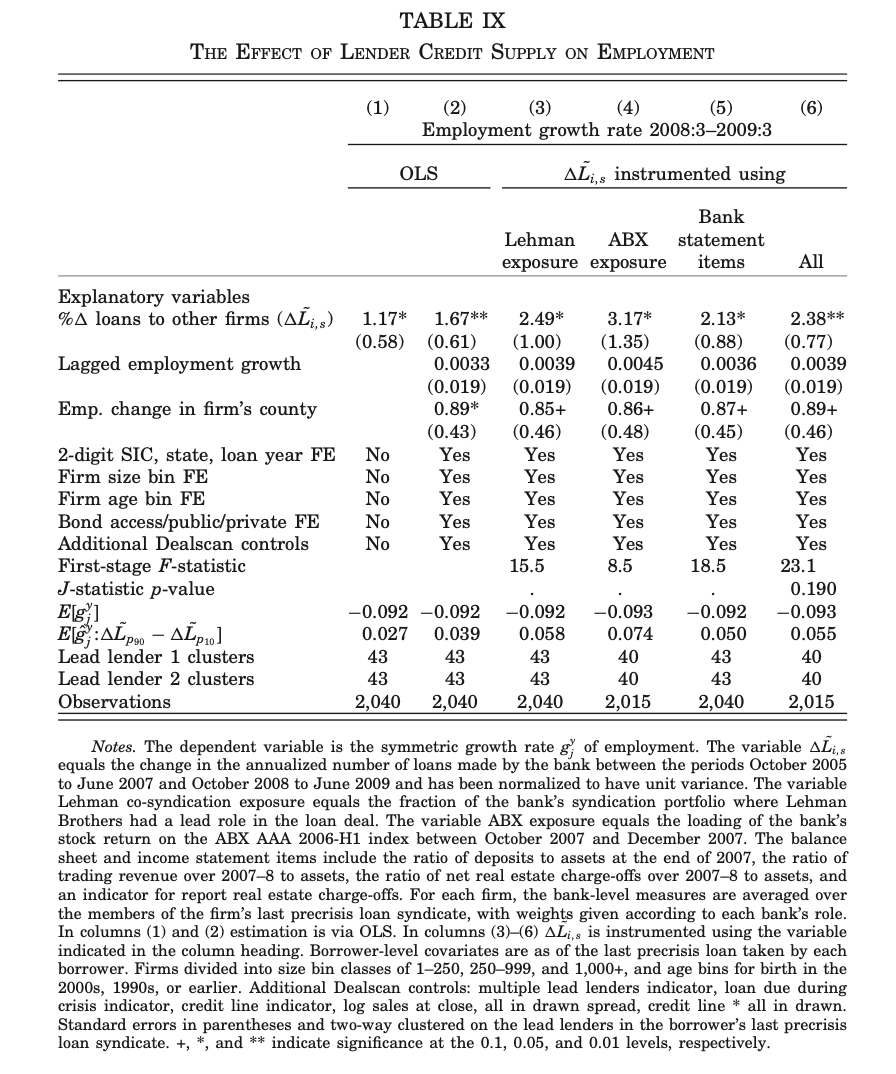
\includegraphics[scale=0.45]{figures/cr_4}
\end{figure}
\end{frame}

\begin{frame}{Aggregate at the regional level}
\begin{itemize}
\item You could be worried that firm-level effects wash out in the aggregate
\item Lehman firms do worse, but non-Lehman firms might do better, nothing much happens in the aggregate
\item One idea is to aggregate at a regional level
\item Why? If you think this competition of Lehman and non-Lehman firms happens in every region, regional outcomes are inclusive of this particular general equilibrium effect
\item Peek and Rosengren (2000) is the seminal paper
\item We will study Huber (2018)
\end{itemize}
\end{frame}


\begin{frame}{Huber 2018}
\begin{itemize}
\item The allies were convinced that the ability of Germany to wage war came from economic centralization
\item From 1948 to 1957, broke up three major banks and created banking zones
\item Firms form ties with banks close to them (Degryse and Ongena 2005)
\item Commerzbank had three HQ's
\item Instrument: Distance to a Commerzbank HQ
\end{itemize}
\end{frame}

\begin{frame}{Results}
\begin{figure}
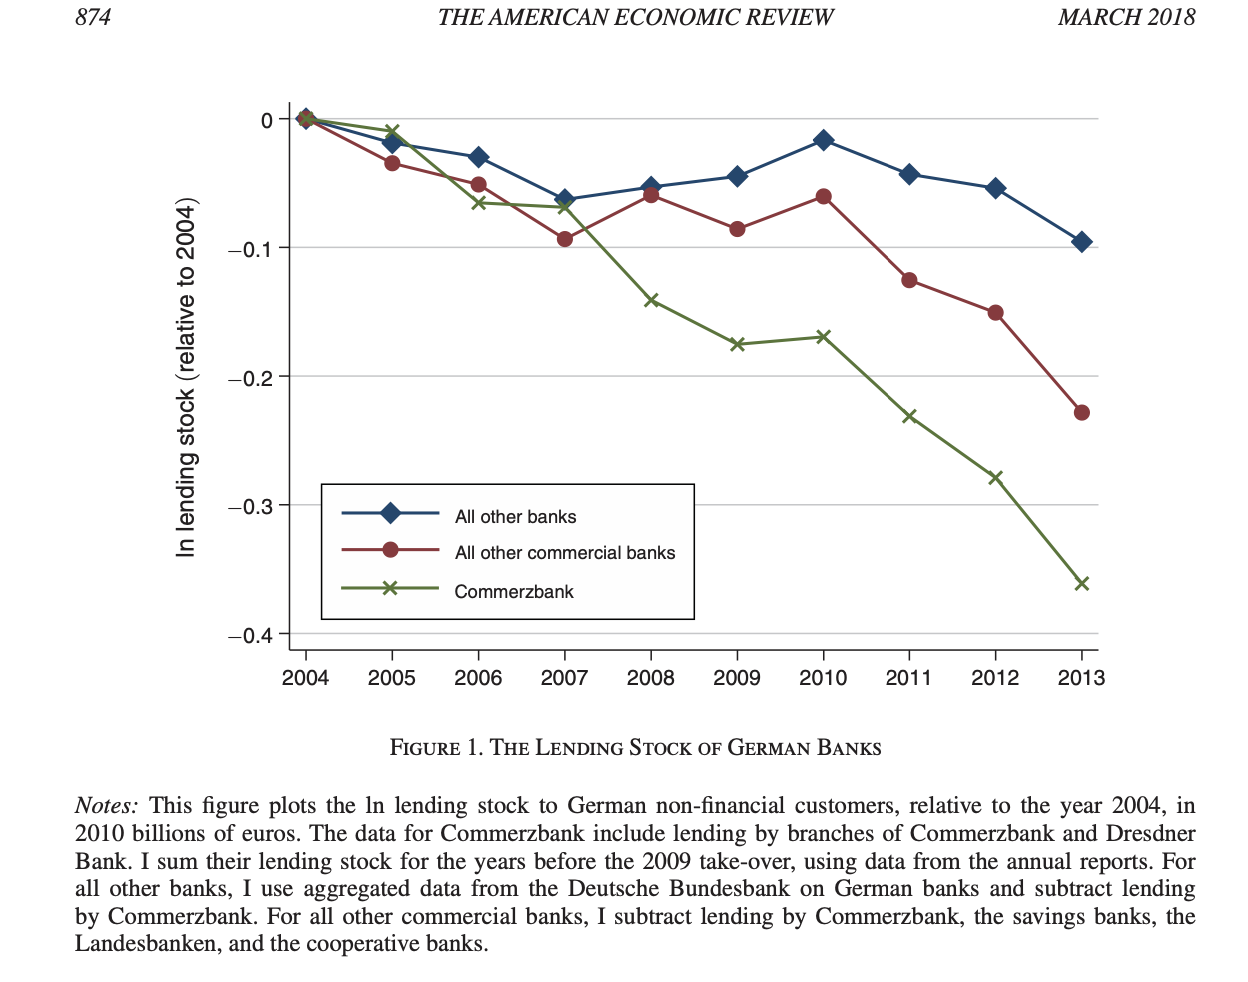
\includegraphics[scale=0.45]{figures/huber_1}
\end{figure}
\end{frame}


\begin{frame}{Specification}
\begin{itemize}
\item Firm-level effects
\[y_{fct} = \zeta  + \beta CBdep_{fc} \times d^{post}_t +\kappa_c\times d^{post}_t + \Gamma' X_{fc} \times d^{post}_t + \gamma_{cf} + \lambda_t + \epsilon_{fct} \]
\item Thoughts?
\end{itemize}
\end{frame}


\begin{frame}{Results}
\begin{figure}
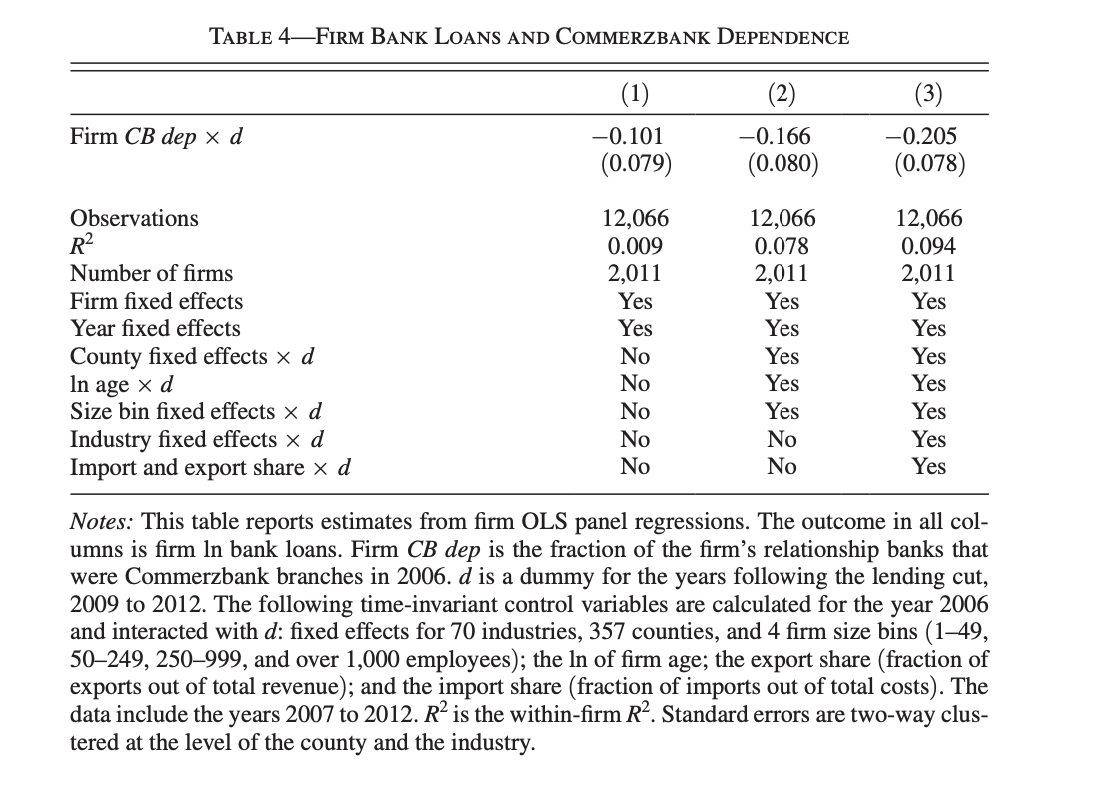
\includegraphics[scale=0.45]{figures/huber_2}
\end{figure}
\end{frame}

\begin{frame}{Results}
\begin{figure}
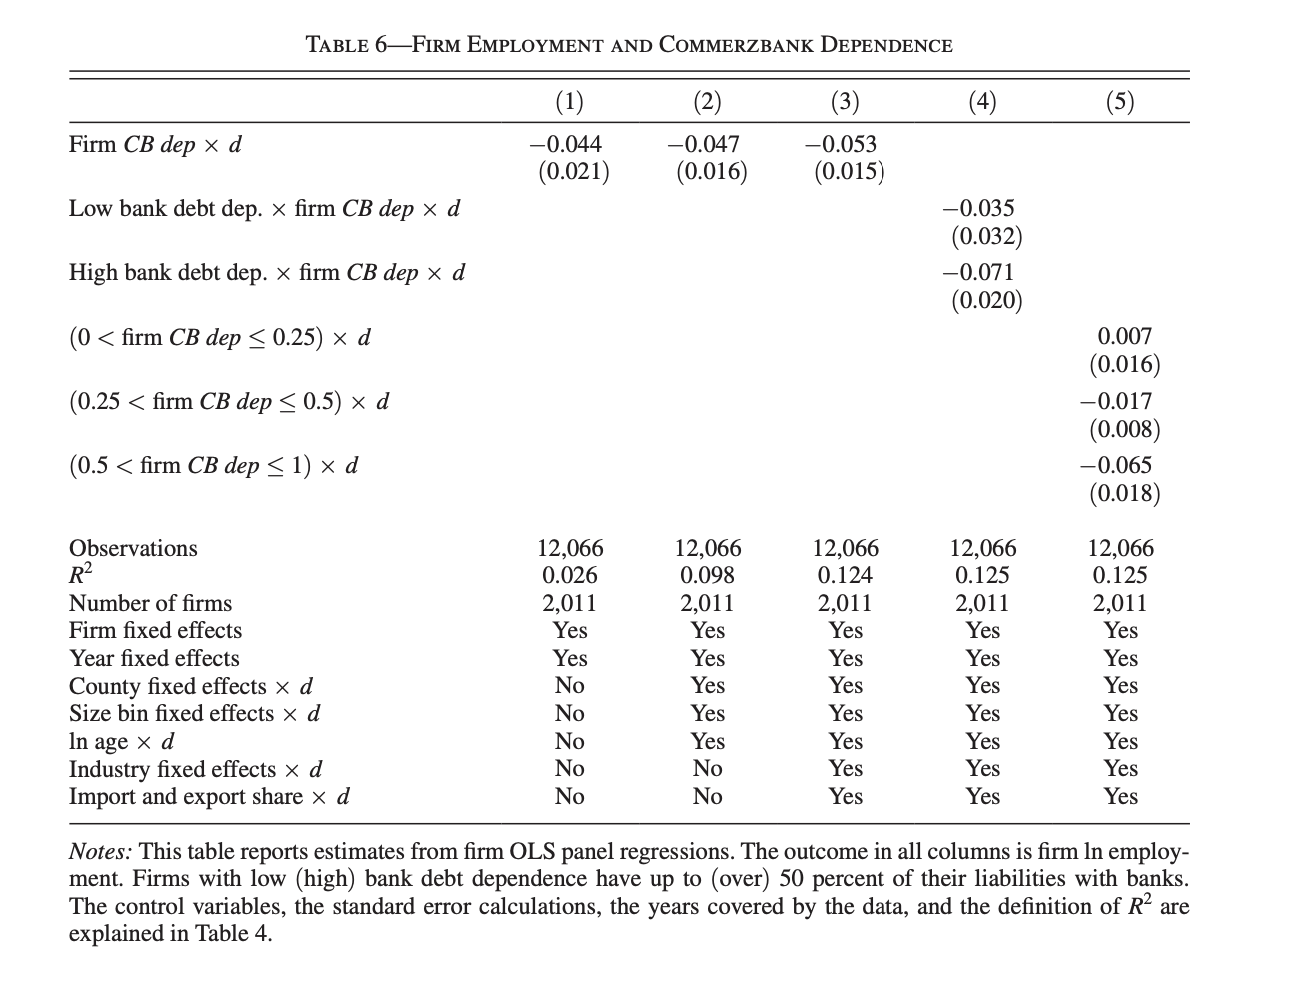
\includegraphics[scale=0.45]{figures/huber_3}
\end{figure}
\end{frame}


\begin{frame}{Results}
\begin{figure}
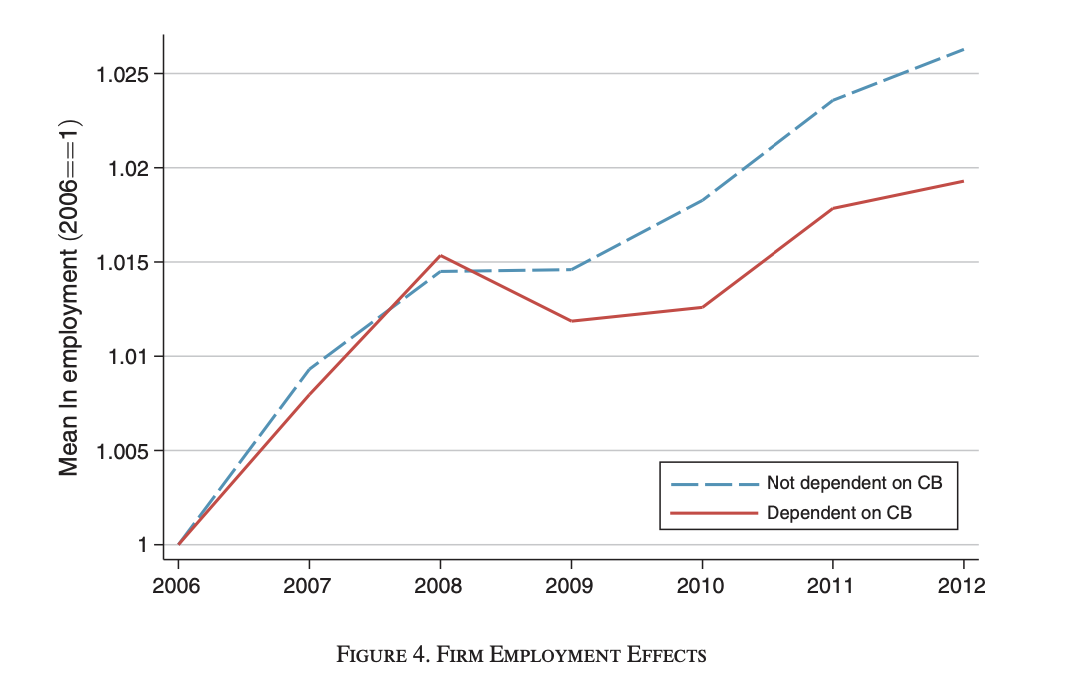
\includegraphics[scale=0.45]{figures/huber_4}
\end{figure}
\end{frame}

\begin{frame}{County Specification}
\begin{itemize}
\item Aggregate at the county level using average exposure
\[y_{ct} = \zeta + \rho \overline{CBdep_c} \times d^{post}_t + \Gamma' X_{c} \times d^{post}_t + \gamma_{c} + \lambda_t + \epsilon_{fct} \]
\end{itemize}
\end{frame}


\begin{frame}{Results}
\begin{figure}
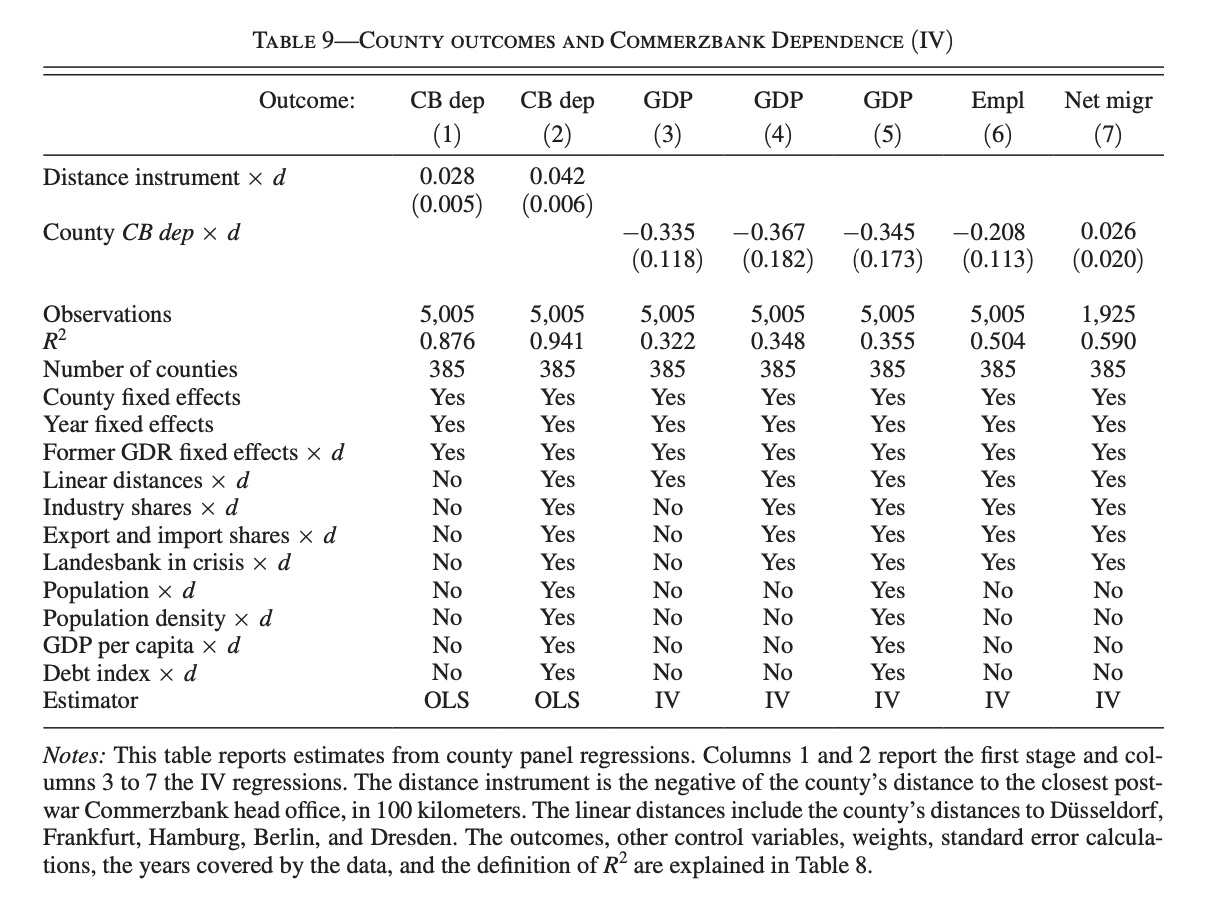
\includegraphics[scale=0.45]{figures/huber_5}
\end{figure}
\end{frame}

\begin{frame}{Indirect Effects}
\begin{itemize}
\item Estimate spillovers in local economies
\[\Delta y_{fc} = \zeta +  \beta {CBdep_{fc}} +  \sigma \overline{CBdep_{fc}}  + \Gamma' X_{fc} +  \xi{fc} \]
\end{itemize}
\end{frame}

\begin{frame}{Results}
\begin{figure}
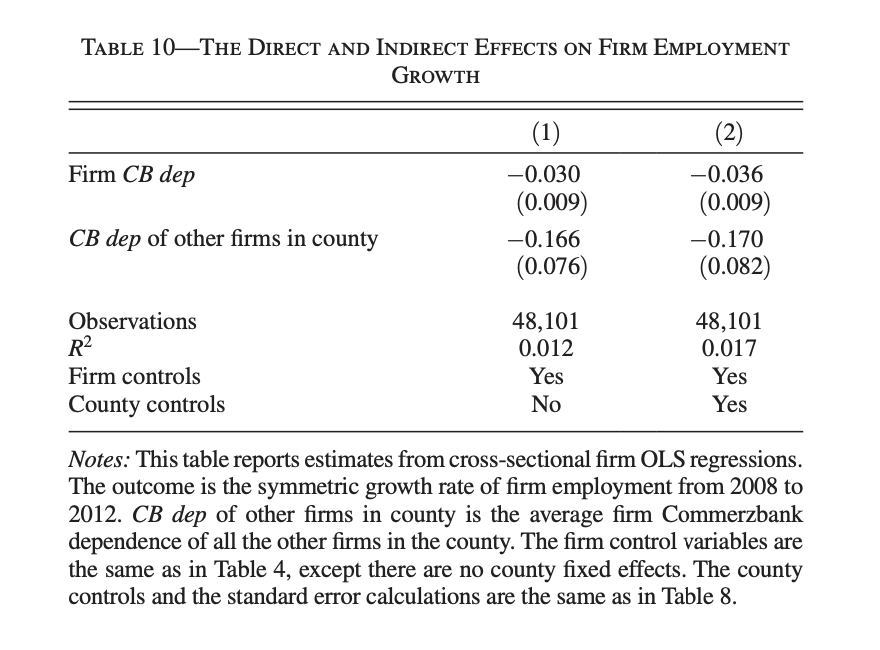
\includegraphics[scale=0.45]{figures/huber_6}
\end{figure}
\end{frame}




\end{document}




